\documentclass[12pt]{article}
\usepackage{lingmacros}
\usepackage{tree-dvips}
\usepackage[utf8]{inputenc}
\usepackage{graphicx}
\usepackage{rotating}
\usepackage[]{authblk}

\title{LitMod python GUI manual}
\author[1]{Ajay Kumar \thanks{SUBITOP (http://www.subitop.eu/home/)}}

%\author[2]{Prof. Manel Fernàndez}
\affil[1]{Group of Dynamics of the Lithosphere, ICTJA-CSIC Barcelona, Spain \\ Email: ajay6763@gmail.com}
%\affil[2]{Group of Dynamics of the Lithosphere, ICTJA-CSIC Barcelona, Spain \\ Email: mfernandez@ictja.csic.es}

\date{March 2017}



\begin{document}

\begin{titlepage}
\maketitle
\end{titlepage}

\section{Introduction}
LitMod is a finite element code which combines potential field, geochemical and seismological data to work out thermo-chemical structure of the lithosphere.\\
This document is a manual for a python based GUI to build the model where the user draws geometry of the bodies in the cross-section and associate physical properties to those bodies.

\section{Python Installation in Windows}
This package uses different libraries from python which does not come pre-installed with stand-alone python installation. So I would recommend installing Anaconda distribution which generally comes with all needed libraries. Anaconda comes with a smart package manager called conda which makes life much easier to install missing packages, this is really handy if you use Windows operating system. Note: anaconda has to be installed in a path with no spaces.This is very crucial.
\begin{itemize}
\item \textbf{anaconda distribution}:Go to anaconda official website and download the anaconda installer according to your platform. Download one with   Python 2.7 version
\end{itemize}
\subsection{Install missing packages}
It might happen that not all packages which are used here, are installed in anaconda distribution.You will know what packages are missing if you run this GUI (To know how to run this GUI go to Start section of this manual). Once you know what packages are missing it's easy to install them using conda package manager which comes with anaconda distribution. Most commonly missing packages are listed below. To install these missing packages just to go to the command prompt in windows and type commands as listed below. If for some reasons it does not work and you still do not have these packages installed just do a simple Google search asking for package name and installation in windows.
\begin{itemize}
\item \textbf{shapely} : conda install -c scitools shapely=1.5.13
\item \textbf{traits} : conda install -c scitools traits
\item \textbf{traitsui} : conda install -c scitools traitsui
\item \textbf{traitsui} : conda install pyqt=4.11.4

\end{itemize}
\section{Python Installation in Linux}
This package uses different libraries from python which does not come pre-installed with stand-alone python installation. Generally, Linux comes with installed python2.7. Now all you have to do is install following packages. Please follow the instructions as follows.
\begin{itemize} 
\item \textbf{Matplotlib}:Matplotlib is a plotting library in python. It needs other packages as well. To take care of everything you only have to do following:
Go to the terminal and type following and hit enter.\\
" sudo apt-get install python-numpy python-scipy python-matplotlib ipython ipython-notebook python-pandas python-sympy python-nose "
\item \textbf{shapely} :Go to terminal and type " sudo apt-get install shapely "
\item \textbf{traits} : Go to terminal and type " sudo apt-get install traits "
\item \textbf{traitsui} : Go to terminal and type " sudo apt-get install traitsui "
\end{itemize}

%%So I would recommend to install Anaconda distribution which generally comes with all needed libraries. Anaconda comes with a smart package manager called conda which makes life much easier to install missing packages, this is really handy if you use Windows operating system.
%%\begin{itemize}
%%\item \textbf{anaconda distribution}:Go to anaconda official website and download the anaconda installer according to your platform. Download one with   Python 2.7 version.
%%Now open a terminal in Linux and go to the folder where you have downloaded the anaconda installer. Make the file executable using chmod 755 "file name" or you can run it like sh "downloaded file name". Then follow the instructions as given.
%%\item \textbf{shapely} :Go to terminal and type "conda install -c scitools shapely=1.5.13"
%%\item \textbf{traits} : conda install -c scitools traits
%%\item \textbf{traitsui} : conda install -c scitools traitsui

%%\end{itemize}


You need an editor to see the python scripts and moreover using a smart editor will help running it as well. I recommend using sublime Text 3 (https://www.sublimetext.com/3). This will take care of path of python libraries and once you open main.py, all you have to do is go to Tools on top right side and click Build or press ctrl+B a window (Fig.~\ref{welcome}) will appear.

\section{Start}
To start the GUI go to the LitMod package folder and run main.py, running which  (Fig.~\ref{welcome}) will appear. Here you have three options. Build model option is to build a model from scratch. Load Model is to load a previously build model and the last option is about help.\\
\begin{figure}
\centering 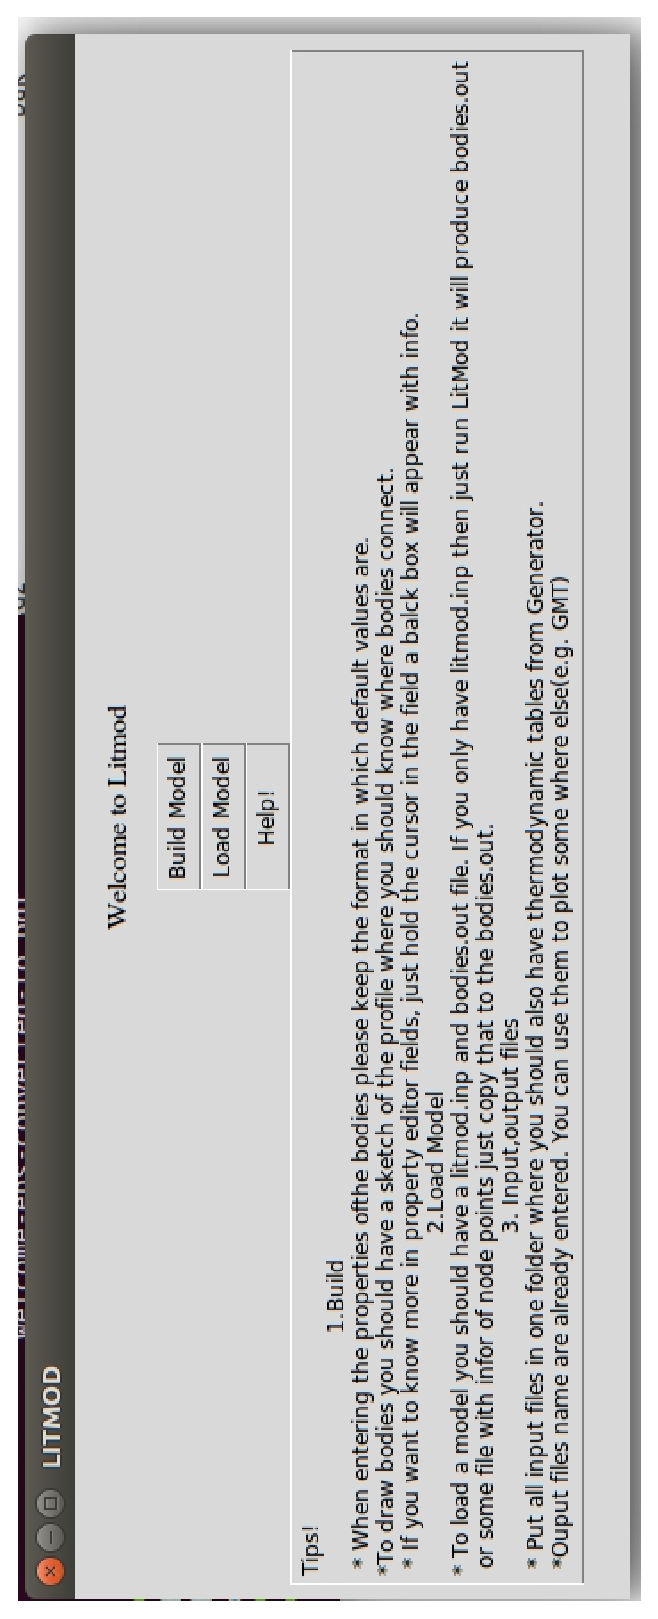
\includegraphics[width=15pc,angle=-90]{./welcome.eps}
\caption{Welcome Page}
\label{welcome}
\end{figure}

\section{Build Model}
Before building a model user should have a clear idea and sketch of the model user wants to build. User should know the vertices's the along which different bodies connected. A model is build from top-to-bottom and every time user wants to exit and wants to save the model, user should close the model by clicking the close Model button on top right. After clicking close model click on the save option which will open a dialog box about some info about the model.\\
After user hits Build Model option a dialogue box appears (Fig.~\ref{build1})
asking for information about the model and another dialogue box asking for digitized file where you already have nodes of the bodies. This digitized file will be plotted in background and you can click on the plotted points. 
\begin{figure}
\centering 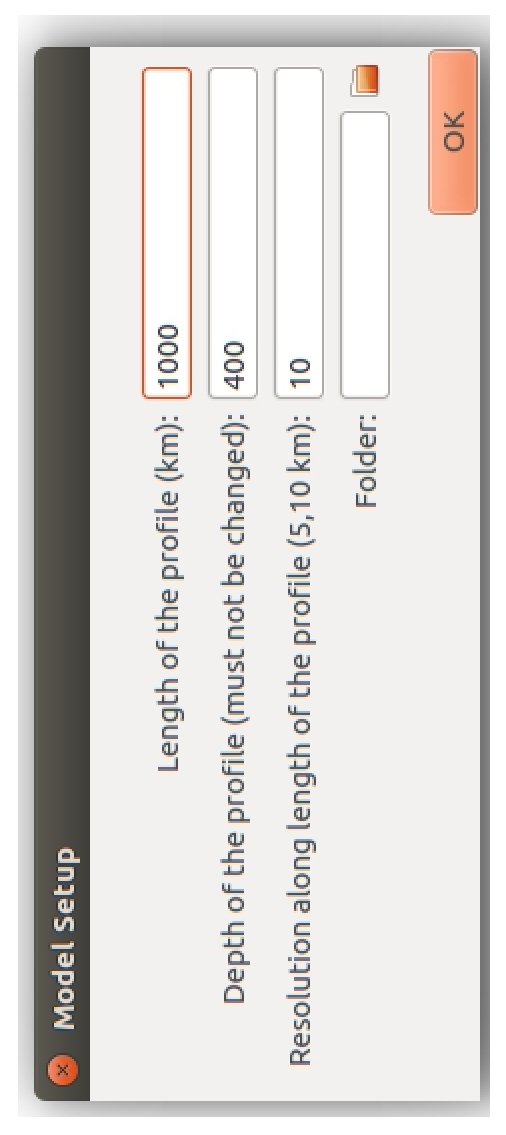
\includegraphics[width=15pc,angle=-90]{./build1.eps}
\caption{Model Setup}
\label{build1}
\end{figure}
\begin{figure}
\centering \includegraphics[width=28pc,angle=-90]{./build2.eps}
\caption{Build Model Window}
\label{build2}
\end{figure}

\begin{itemize}
\item \textbf{X length}: This the length of the profile in km.
\item \textbf{Y length}: This the depth of the profile in km. It must be 400km, so it must not be changed.
\item \textbf{Dir} : Here user selects the folder in which observable files are put and it becomes the working folder for LitMod. All the outputs and files are stored in this folder.
\end{itemize}
After the user hits OK button build model window will appear (Fig.~\ref{build2}). Here the user has different option.

\subsection{Add Body}
\begin{figure}
\centering 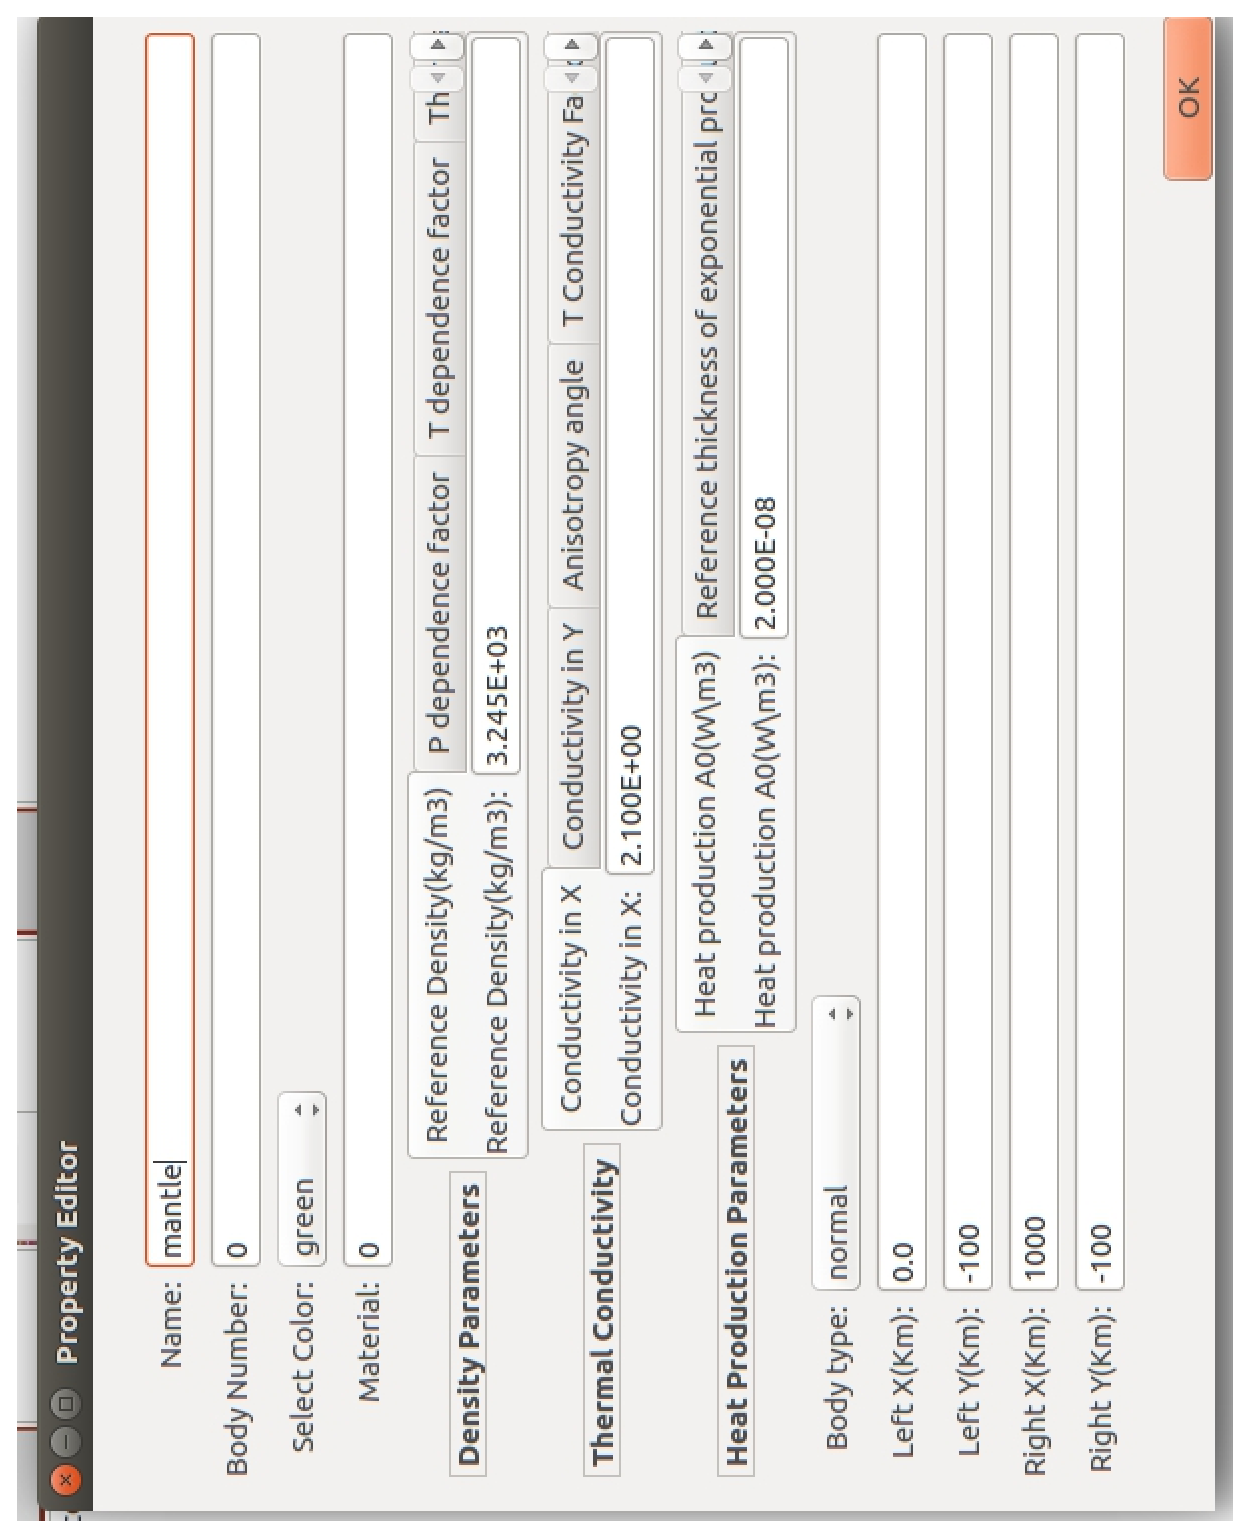
\includegraphics[width=25pc,angle=-90]{./build_propety.eps}
\caption{Body property editor}
\label{body_property}
\end{figure}
Bodies are added from top to bottom, each body is drawn left to the right.To add a body press the add button on the window (Fig.~\ref{build2}) which will open a dialog box asking for information about the body (Fig.~\ref{body_property}).\\ 
**Please note that format in which default values appear should be maintained.
\textbf{Fields description}
\begin{itemize}
\item \textbf{Name}     : Name of the body. Just for your reference
\item \textbf{Body number} : Index of the body starting from the top.
\item \textbf{Material} :Type of material of the body
\item \textbf{Body type}: if you are adding a body which is new, this option should be normal. If you are splitting a body change this option to split. If you are adding an anomaly change this option to type of anomaly you are adding (thermal or seismic).
\item \textbf{Xs Ys}: start point of the body. Remember it has to be the left most point. 
\item \textbf{Xe Ye}: end point of the body. Remember it has to be the right most point. 
\end{itemize}
Once the user is done with adding properties user should hit OK and control will be back to the plotting area where the start and end point of the body will be already drawn in color chosen.
\begin{itemize}
\item \textbf{to add point}: Middle click
\item \textbf{to delete current point}: double left click
\item \textbf{to close body}: right click
\end{itemize} 
\subsection{Delete body}
The user can delete the last body entered by clicking on the delete button. Let us say a user has drawn three bodies. To delete second body first user has to delete the third body.
\subsection{Change shape of the bodies}
To move the vertices's of the drawn bodies user can click on shape button. After clicking this button a separate plot will appear where all bodies will be drawn as points. Now user can move these point by left click drag, changes can be saved with right click.Once you have saved changes close the window and come back to the main window and hit plot button which will update the changes. Once user us satisfied with the shape to save changes click right button on the mouse close the window and hit plot button. This function will only work after you have closed your model. 
\subsection{Edit properties}
To edit properties of a body already drawn click on edit button and a dialog box will appear asking for the index of the body you want to edit. *NOTE: with this option user can only edit the properties other than start and end point of the body.
\subsection{Split body}
This function allows the user to split a body into two. This function should be used with a lot of care. The user should know exactly where to start split and where to end and it is advisable that start and end nodes points are already in the body to be split.  
\subsection{Run model}
To run a model first you have to save the model by clicking on the save button, but before that, your model should be closed. You should also put the observables file (topography, bougeur, geoid, free air, heat flux) in the same folder and composition files (e.g. 80 81 88 99 etc) which you have associated with the bodies in your model.\\ 
*Note:To run a model you should have LitMod program executable for windows or linux based on your system. Executable for Linux is provided with the distribution . Name of these executables should be LITMOD\_V4\_VS\_Windows for windows and should be in LITMOD\_package folder and for Linux it should be in same folder with name LITMOD\_V4\_VS\_Linux.
\section{Load Model}
This option lets the user load previously build models. To load models user need file 1. litmod.inp file, which input file to the LitMod program and 2. bodies.out , this file contains nodes point of the bodies in the model. Units of nodes points in bodies.dat are in kilometers. If you have a litmod.inp file which is not built in this GUI than the user should first run that input file in LitMod code which will produce bodies.dat file with bodies nodes in kilometers and then that file can be  used to load the model in this GUI.

\section{Anomalies}
In this GUI anomalies are added on top of the completely closed profile. At the moment you can not use shape function for anomalies. if you want to edit a anomaly only solution at the moment is to delete the one you want to edit and add it again.\\
In case where you have loaded a profile with anomalies and you want to edit the normal bodies, first delete  anomalous bodies and go ahead.\\

*Note : this is very important to do things in sequence as you choose for them. Control sequence of the GUI very static which will be made dynamic in future versions. 


  



\section{Miscellaneous}



\end{document}
